\subsection{Related work}

Traffic fluency monitoring and jam detection is part of traffic
control in all major cities and the real time information about road
network fluency is of interest to all network users and traffic
related authorities. Over the last years, several different methods
for detecting jams have been created. In many cities traffic is
monitored via road side cameras detecting fluency in the most
important channels of the network and sends the image to authorities
and web services. Another increasingly popular method for detecting
jams is by traffic message channels (TMC) that collect information
about road network status from roadside sensors and vehicles and
transmits the information via radio signals to the end user. TMC
information is most commonly used in navigators, both on inbuilt
vehicle navigating systems and separate navigator
devices.\footnote{\url{http://www.tisa.org/technologies/tmc/}} Over
the past few years also different smartphone applications, such as
Waze or Inrix have emerged on the market. In these applications
information gathering is commonly done either with the vehicles
connected to the system or by the users who report their journey
conditions around them. Different applications provide different type
of information, usually including one or several of the following
information types: jams, weather, road work and accidents.  What is
common to all known methods for detecting jams, no service is provided
specifically to the public transport users as most services are
targeted for private vehicle drivers and the authorities. Based on our
surveys no service is being used specifically to public transport nor
uses the delay information of public transport vehicles, which makes
the traffic jam detection module an unique tool.

\subsection{Component Description}

The jam detection module frequently polls vehicle location compared to
the scheduled location from the Helsinki public transport service. The
module analyses the vehicle situation and detects where there are
traffic jams in the certain transportation authority’s transportation
area. The interface returns always the current jam situation, so
client does not need to keep the jams in memory.

The module detects the jams based the tram location, taking into
notice the delay and how fast it increases. Also, the jam is only
detected if there are several vehicles filling the same criteria
within the same area.  


The module provides information about the nearest stop to the detected
jam and also the previous stop from where the affected vehicles have
come from. Based on this information current traffic situation is
visualized on the application.  All of Helsinki city tram network can
be drawn on the map, but only lines that are currently affected by
trams are shown on the map at each time. If no jams are detected in
between two stops, this interval is shown with green colored line. If
a jam is detected between stops, the interval is shown with red
colored line. Image \ref{fig:tjd_screenshot} shows a screenshot of the application on how the
jams are presented in Helsinki city center during the trial.

\begin{figure}
\centering
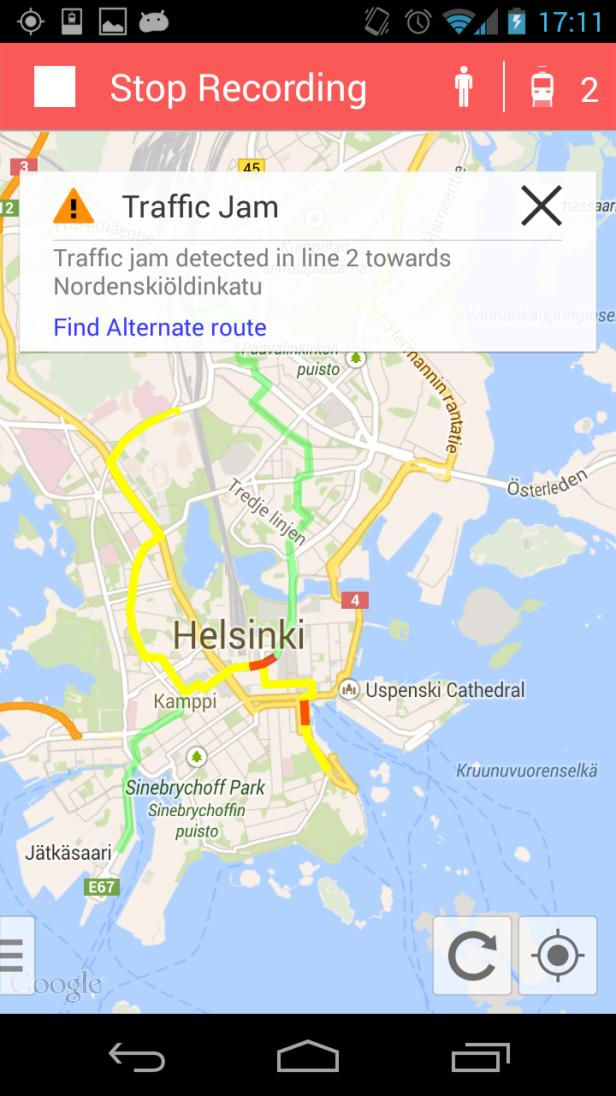
\includegraphics[width=0.3 \textwidth]{img/tjd/screenshot.jpg}
\caption{Visualization of the current traffic situation in Helsinki based on Jam detection}\label{fig:tjd_screenshot}
\end{figure}

\subsubsection*{Architecture Description}

The JamDetector module simplified architecture is visualized in the
Figure \ref{fig:tjd_architecture}. The public transportation systems
generally differ in each city or area in multiple ways in the
available data and data formats. The different public transportation
systems are isolated in the module and configurable using the Spring
Framework.

\begin{figure}
\centering
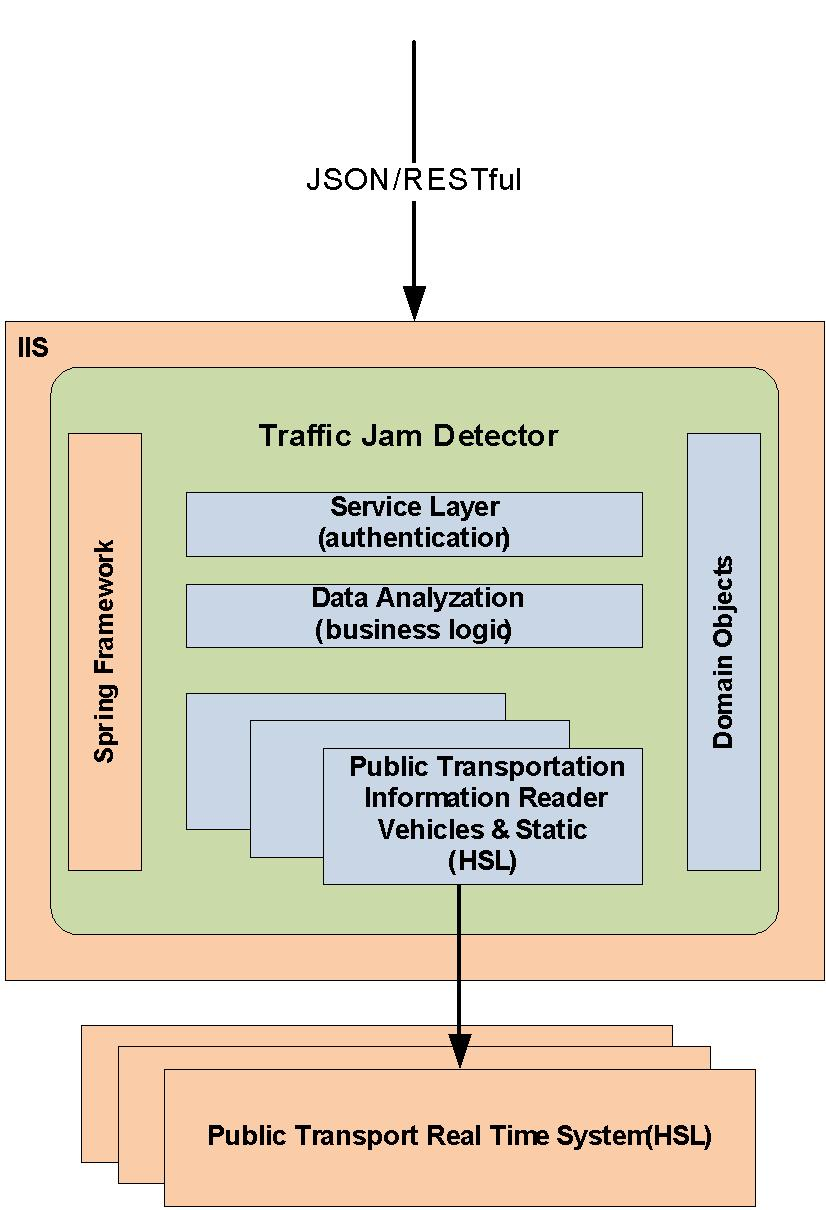
\includegraphics[width=0.5 \textwidth]{img/tjd/architecture.jpg}
\caption{Traffic Jam Module Architecture}\label{fig:tjd_architecture}
\end{figure}

\subsubsection*{Live+Gov SaaS solution compatibility}

The JamDetector follows Live+Gov SaaS architecture. This means that
all connecting clients are authorized. Also the JamDetector provides
the heart beat (health check) information to the SaaS service and
sends the application log to the service.  

\subsection*{API description}

The API lists the jams detected in the certain public transportation
area in JSON format. The jam object contains information about the
vehicles participating the detected jam and vehicle’s nearest
stop/station. This information can be used to visualize the jam
location for the users.

\subsection*{Data structure}

The data structure of the JSON-message is described in figure \ref{fig:tjd_datastructure}.

\begin{figure}[htbp]
\centering
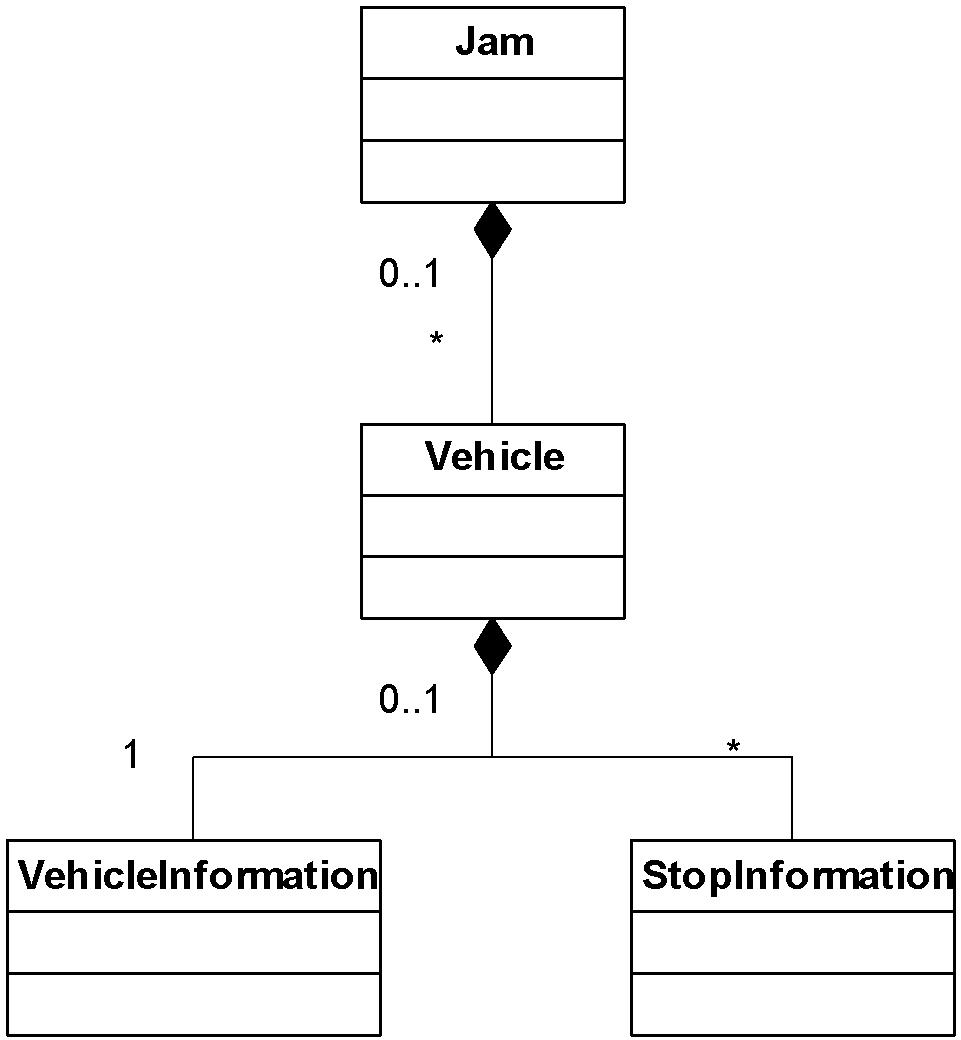
\includegraphics[width=0.5 \textwidth]{img/tjd/data_structure.jpg}
\caption{JSON data structure}\label{fig:tjd_datastructure}
\end{figure}

Example of a given message:

\begin{verbatim}
URL /jamdetector/JamService.svc/jams/hsl

[ { "Id" : 0,
    "IsJam" : true,
    "SlowVehicles" : [ { "CumulativeDelay" : 13,
          "NextStop" : { "Code" : "1301453",
              "Latitude" : 60.197929999999999,
              "Longitude" : 24.876580000000001,
              "Name" : "Laajalahden aukio"
            },
          "PreviousStop" : { "Code" : "1301455",
              "Latitude" : 60.195390000000003,
              "Longitude" : 24.873429999999999,
              "Name" : "Tiilimäki"
            },
          "Stop" : { "Code" : "1301455",
              "Latitude" : 60.195390000000003,
              "Longitude" : 24.873429999999999,
              "Name" : "Tiilimäki"
            },
          "Vehicle" : { "Delay" : 13,
              "Id" : "RHKL00076",
              "IsOnStop" : false,
              "Latitude" : 24.873405999999999,
              "LineDirection" : 2,
              "LineId" : "1004",
              "Longitude" : 60.195535999999997,
              "NextStopIndex" : 2,
              "Time" : "20140116-102700",
              "Timestamp" : "/Date(1389860820413+0200)/"
            }
        },
        { "CumulativeDelay" : 72,
          "NextStop" : { "Code" : "1240419",
              "Latitude" : 60.203020000000002,
              "Longitude" : 24.96584,
              "Name" : "Kyläsaarenkatu"
            },
          "PreviousStop" : { "Code" : "1230410",
              "Latitude" : 60.204529999999998,
              "Longitude" : 24.96998,
              "Name" : "Toukoniitty"
            },
          "Stop" : { "Code" : "1230410",
              "Latitude" : 60.204529999999998,
              "Longitude" : 24.96998,
              "Name" : "Toukoniitty"
            },
          "Vehicle" : { "Delay" : 82,
              "Id" : "RHKL00065",
              "IsOnStop" : false,
              "Latitude" : 24.968769999999999,
              "LineDirection" : 2,
              "LineId" : "1006",
              "Longitude" : 60.203980999999999,
              "NextStopIndex" : 3,
              "Time" : "20140116-102700",
              "Timestamp" : "/Date(1389860820405+0200)/"
            }
        }
      ],
    "SlowVehiclesInJamCount" : 2
  } ]
]
\end{verbatim}

In this example the JamDetector has detected one jam and there are two
vehicles in the jam. In addition to the vehicle information the next,
previous and nearest stop information is returned. The jam location
can be approximated either from the participating vehicle locations or
stop locations.  The interface contains more information than the
current clients require. This is for debugging and possible
visualization purposes. For example vehicle’s line information is such
information.

If there are no jams currently detected, the interface returns:
\begin{verbatim}
[]
\end{verbatim}


\subsection{Evaluation}
The module development begun with evaluating different methods for
creating the detection algorithms and creating a way to detect jams
reliably. The tram location data from Helsinki provides reliable
information about the delay of a vehicle in real time and was
considered the most efficient and reliable source of data for the jam
detection.

A comprehensive and reliable detection algorithm was created through
experimenting in the early stages of the module development. The
parameters to be used were searched the most suitable values through
thorough consideration in order to generate reasonable and accurate
alerts that would correspond with the logical situation in traffic and
would fit in the definition of a jam. After some weeks of monitoring
the detections, the defined values were also re-evaluated and
re-defined before the first pilot based on the previous observations. 

Based on the first trial results, the amount of detected jams is seen
relatively high, on average 3 jams were received on each time the API
was called. This would indicate the parameters needing to be set
tighter in the future if only greater jams are wanted to be
detected. When evaluating the accuracy it was quickly discovered that
validating the detection is rather challenging when not having the
possibility to verify the situation on site. User questionnaires
showed that no users were travelling in the areas where alerts were
given at the time of the alert and therefore they could not reliably
state their opinion about the accuracy of alerts. Also, no known major
jams took place during the trial in the pilot area and therefore
manual validation could not be done during the trial. Manual
comparison to other known services providing jam alerts was done. In
all cases the detected jams were of a short duration, mainly less than
a minute and therefore no reliable statement about accuracy could be
done at this stage. In the comparison we used two popular services:
Waze\footnote{\url{http://www.inrixtraffic.com/}}, which is a mobile
application providing traffic data in over 30 countries and
V-traffic\footnote{\url{http://www.v-traffic.fi/}} , a national
service in Finland for providing traffic data in major cities. Based
on the comparison to other services the results seem promising as
alerts were given in the same areas at the same time, only with minor
differences.

When comparing the module to existing services it is obvious that
there are existing systems that provide information with more
geographical coverage and collect the data from greater number of
sources. Thus, these services also provide more alerts as they also
cover roads that are not included in the current module coverage, the
Helsinki tram network. What needs to be addressed when comparing the
module to existing services is that the other services do not focus on
public transport and using only these services would not help to meet
the requirements of the mobility use case in full. However, the
possibility to support the jam detection module with existing services
needs to be further studied. 

We believe that when expanding the data to also cover other public
transport vehicles, the coverage in the module will increase and the
quality and the usefulness of the module improves. For example in the
Helsinki region, all public transport busses, trams, trains and the
ferry will be covered in the new public transport information system
to be implemented in 2016. Then the module will provide a much better
service with greater geographical coverage and expanded
fleet. Unfortunately at the time of development, location data is not
yet available for other vehicles than trams but the possibility to
include these vehicles in the jam detection has been taken into notice
from the start.

As no reliable evaluation is possible at this stage we will continue
validating the module, analyzing the results and developing the
algorithms. This process will continue until the final trial where
improvements and reliable accuracy of the module are hoped to have
been achieved.

%%% Local Variables:
%%% mode: latex
%%% TeX-master: "../D1-2"
%%% End:
